\documentclass[11pt,xcolor={svgnames},aspectratio=169,usepdftitle=false,notheorems]{beamer}
%===========================================================
% DOCUMENT
%===========================================================
\usepackage{rafa_style_beamer}  % Loads my formatting 

\usepackage{dirtree}

\addbibresource{../matlab_intro.bib}

\title{Introduction to Matlab}
\subtitle{Lesson 01 --- Matlab Syntax}

\author{Rafael Serrano-Quintero}

\institute{Department of Economics \\ University of Barcelona}
\date{}

\begin{document}

\VerbatimFootnotes

\maketitle

\section{Preliminaries}

\begin{frame}
    \frametitle{Preliminaries}
    \textbf{\alert{The Course}}
    \begin{itemize}
        \item Introduction to Matlab Programming
        \item Check the \href{run:../syllabus/syllabus.pdf}{syllabus}
    \end{itemize}
    \textbf{\alert{Me}}
    \begin{itemize}
        \item \href{rafserqui.github.io}{Rafa Serrano-Quintero} \href{mailto:rafael.serrano@ub.edu}{(rafael.serrano@ub.edu)}
        \item Office hours: Any time. Send me an email and we can arrange a meeting.
    \end{itemize}
    \textbf{\alert{You}}
    \begin{itemize}
        \item A quick roundtable of names, interests, and coding background.
    \end{itemize}
\end{frame}

\begin{frame}
    \frametitle{What will we cover?}
    \begin{enumerate}
        \item Matlab preliminaries. 
            \begin{itemize}
                \item First interactions. Script vs Command Window.
                \item Creating Variables. Basic Operations. Arrays and Matrices.
                \item Control Flow. Plots. Functions.
            \end{itemize}
        \item Importing and manipulating data. Polynomial fit and evaluation. Nonlinear least squares.
        \item Basics of root finding, numerical differentiation and integration.
        \item Basics of numerical optimization.
    \end{enumerate}
\end{frame}

\begin{frame}
    \frametitle{Syllabus Highlights}
    \textbf{\alert{What you have to do}}
    \begin{enumerate}
        \item Two problem sets
        \item In class solutions
        \item Final exam (take-home)
    \end{enumerate}
\end{frame}
    
\begin{frame}
  \frametitle{Syllabus Highlights --- Materials}
    \begin{itemize}
      \item \href{https://www.elsevier.com/books/matlab/attaway/978-0-323-91750-6}{\fullcite{attaway2019matlab}}
        \item \href{https://people.lu.usi.ch/gruberp/MatlabMasterScript.pdf}{Peter H. Gruber --- Script Solving Economics and Finance Problems with MATLAB}
        \item \href{https://quantecon.org/lectures/}{QuantEcon Lectures.} These are written for Python and Julia but many ideas port to Matlab easily.
        \item \href{https://cheatsheets.quantecon.org/index.html}{QuantEcon Cheatsheet} ---  for Matlab, Python, and Julia.
    \end{itemize}
\end{frame}

\begin{frame}[c]
  \frametitle{What Matters}
 \begin{itemize}
  \item Not where you end up relative to your classmates but where you end up relative to your current self!
  \item Most of you never have programmed, and that's \alert{\textbf{fine!}} 
  \item What is programming? Problem solving!
  \item Programming in one diagram: 
 \end{itemize} 

 \begin{center}
   \usetikzlibrary{positioning}

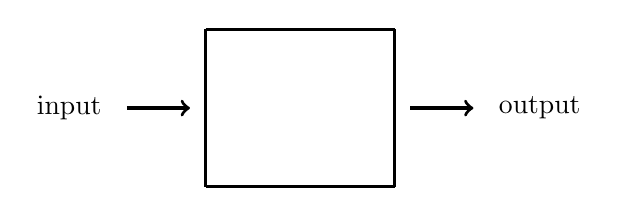
\begin{tikzpicture}[scale=0.2]
  
  \node[left] at (0,5) {input};

  % Arrow
  \draw[very thick,->] (1,5)--(5,5);

  % Square
  \draw[very thick,-] (6,0)--(6,10);
  \draw[very thick,-] (6,0)--(18,0);
  \draw[very thick,-] (6,10)--(18,10);
  \draw[very thick,-] (18,0)--(18,10);

  % Arrow
  \draw[very thick,->] (19,5)--(23,5);
  \node[right] at (24,5) {output};
\end{tikzpicture}


 \end{center}
 
\end{frame}

\begin{frame}[c]
  \frametitle{Why do we need programming?}
  \begin{exercise}
   Suppose a firm faces a linear demand curve such as $P = a - b Q$ and the firm's cost function is given by $C(Q) = cQ + d$ where $P$ is price, $Q$ quantity, and $a,b,c,$ and $d$ are positive real constants. Find the optimal quantity to produce.
  \end{exercise}
  \pause
  \begin{solution}
   Deriving the profit function $\Pi = PQ - C(Q)$ with respect to $Q$, we find
   \[
     \frac{\partial \Pi}{\partial Q} = -2b Q + (a - c) = 0 \Rightarrow Q = \frac{a - c}{2b} 
   \]
  \end{solution}
  
\end{frame}

\begin{frame}[c]
  \frametitle{Why do we need programming?}
 \begin{exercise}
   Suppose now the demand curve is $P = 10 - Q^{1/2} - Q^{1/5}$ and $C(Q) = cQ + d$.
 \end{exercise}

 \begin{solution}
   Now the profit function is $\Pi = 10Q - Q^{3/2} - Q^{6/5} - cQ - d$ and the FOC is 
   \[
     \frac{3}{2} Q^{1/2} + \frac{6}{5}Q^{1/5} + c - 10 = 0 
   \]
   How do we solve this \textit{``by hand''}? Say $10 - c = 1 \Rightarrow c = 9$. Then, we can define $G(Q) \equiv \frac{3}{2} Q^{1/2} + \frac{6}{5}Q^{1/5} - 1$ and find $G(Q) = 0$.
   \begin{itemize}
    \item $G(0) = -1$
    \item $G(1) = 1.7 > 0$
   \end{itemize}
   We know there exists some $q\in(0,1)$ such that $G(q) = 0$. But we cannot say much more analytically!
 \end{solution}
 
\end{frame}

\begin{frame}[fragile]
  \frametitle{Why do we need programming?}
  \textit{In Matlab, we could find the solution with two lines of code:}
 \begin{lstlisting}
gq = @(q) (3/2) .* q.^(1/2) + (6/5) .* q.^(1/5) - 1;
qopt = fzero(gq, 0.5);
qopt = 
      0.050915576865381714788405531635362
 \end{lstlisting}
\end{frame}

\begin{frame}[c]
  \frametitle{Why do we need programming?}
  
  \begin{itemize}
    \item Econometrics/Empirical analysis.
    \item Applied general equilibrium.
    \item Complement for theory. Substitute when looking at very complex models.
    \item We will use Matlab but many things translate to other languages (e.g. Python, Julia, R\ldots).
    \item Try to learn \alert{\textbf{concepts!}} 
  \end{itemize}

\end{frame}

\section{First Time Opening Matlab}

\begin{frame}
    \frametitle{First Time Opening Matlab}
\begin{figure}
    \centering
    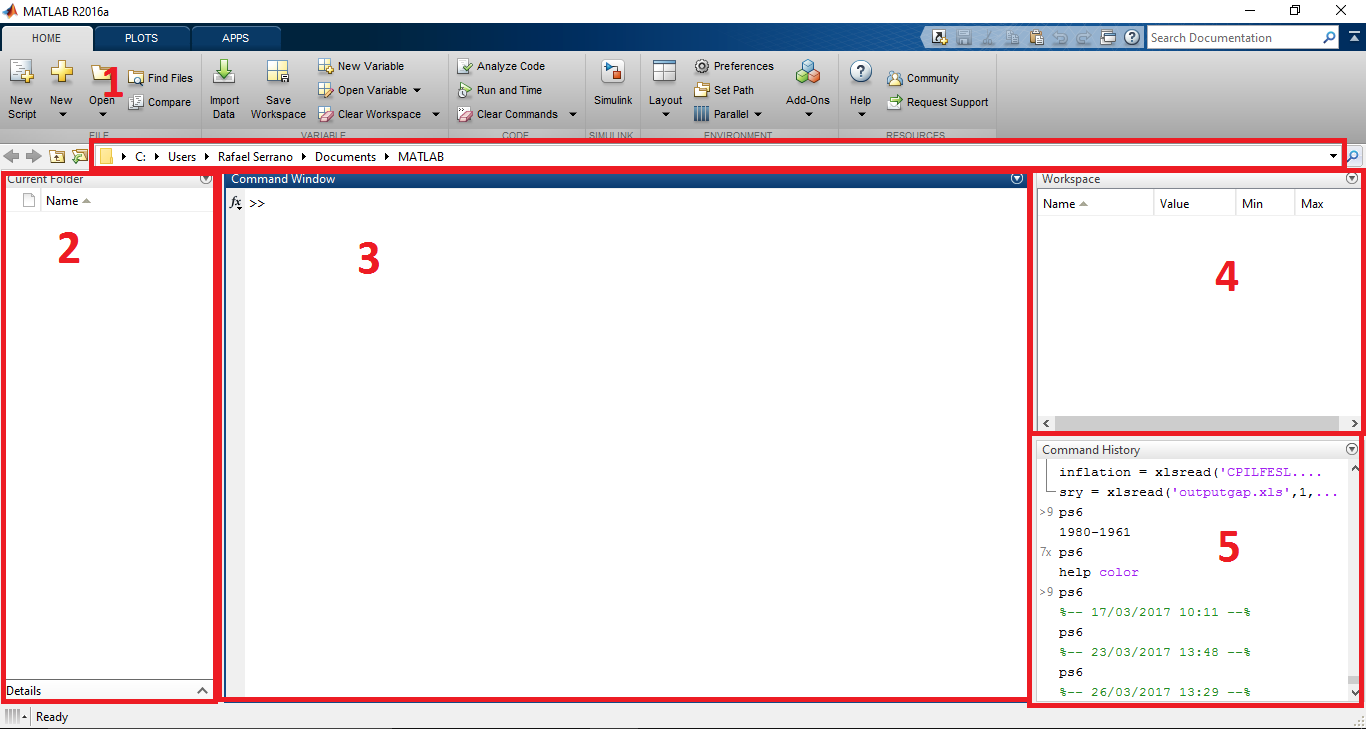
\includegraphics[width = 0.8\textwidth]{../figures/matlab_initial.PNG}
    \caption{Matlab's Interface}
    \label{fig:matlab_interface}
\end{figure}
\end{frame}

\begin{frame}[fragile]
    \frametitle{Working Directories}
\begin{itemize}
    \item For Matlab to find files and know where its working, it needs a \alert{\textbf{working directory}}.
    \item A directory is a folder that has relationships to other folders.
\end{itemize}
\dirtree{%
    .1 matlab-class.
    .2 slides.
    .2 codes.
    .2 problem-sets.
    .3 ps1.
    .3 ps2.
}
\begin{itemize}
    \item Say we want to run codes in the \verb;codes; subfolder. Then, we must \alert{\textbf{point to where}} the folder is.
\end{itemize}
\end{frame}

\begin{frame}[fragile]
    \frametitle{Working Directories}
\begin{columns}
    \begin{column}{0.2\textwidth}
        \dirtree{%
            .1 matlab-class.
            .2 slides.
            .2 codes.
            .2 problem-sets.
            .3 ps1.
            .3 ps2.
        }
    \end{column}
    \begin{column}{0.8\textwidth}
        \begin{itemize}
            \item In this example \verb;matlab-class; is called the \alert{\textbf{parent directory}}.
            \item But \verb;problem-sets; is the parent directory of \verb;ps1; and \verb;ps2;.
            \item The \alert{\textbf{working directory}} refers to the directory on your computer that Matlab assumes is the starting place for all paths that you construct or try to access.
        \end{itemize}
    \end{column}
\end{columns}
\end{frame}

\begin{frame}[fragile]
    \frametitle{Paths}
\begin{columns}
    \begin{column}{0.2\textwidth}
        \dirtree{%
            .1 matlab-class.
            .2 slides.
            .2 codes.
            .2 problem-sets.
            .3 ps1.
            .3 ps2.
        }
    \end{column}
    \begin{column}{0.8\textwidth}
        \begin{itemize}
            \item Suppose \verb;matlab-class; is in \verb;C:\Users\Rafa\Documents\matlab-class\;.
            \item That is called the \alert{\textbf{absolute path}}.
            \item The absolute path of \verb;slides; is \verb;C:\Users\Rafa\Documents\matlab-class\slides\;.
            \item The \alert{\textbf{relative path}} is a path relative to the working directory.
            \item The relative path of \verb;ps1; would be \verb;./problem-sets/ps1/;.
            \item Matlab understands relative paths.
        \end{itemize}
    \end{column}
\end{columns}
\end{frame}

\begin{frame}[fragile]
    \frametitle{The Two Most Useful Commands}
\begin{itemize}
    \item If you make some mistake and need Matlab to stop, \verb;Ctrl+C; on the command window.
    \item When you do not know how a command works or what it does, use \verb;help;.
\end{itemize}
\end{frame}

\section{Scripts vs Command Window}

\begin{frame}
    \frametitle{Scripts vs Commands}
\begin{itemize}
    \item The \alert{\textit{command window}} allows us to evaluate commands we type.
    \item \alert{\textit{Scripts}} are \textit{recipes} that can be saved. Useful for:
    \begin{itemize}
        \item Reproducing a set of codes \alert{exactly} in the same order
        \item Automating tasks
        \item Correcting mistakes in long tasks
    \end{itemize}
    \item A script is evaluated sequentially line by line.
\end{itemize}
\end{frame}

\begin{frame}[fragile]
    \frametitle{Scripts vs Commands}
    \begin{itemize}
        \item To start a new script:
        \begin{itemize}
            \item \verb;Home -> New Script;
            \item Type \verb;edit; in the command window
        \end{itemize}
        \item Write comments with the symbol \verb;%; 
        \item Everything after a \verb;%; will not be processed by Matlab
        \item A block of comments is defined within \verb;%{ %};
    \end{itemize}
\end{frame}

\begin{frame}[fragile]{Script Example}
\begin{lstlisting}
clear all
close all 
clc

% This is a comment

%{
    This is a block of comments. Everything within the two symbols is not processed by Matlab. Useful to define headers or helps for user defined functions.
%}
\end{lstlisting}
\end{frame}

\section{Creating Variables}

\begin{frame}
    \frametitle{Creating Variables}
    \begin{itemize}
        \item We can \alert{\textbf{assign}} values to a variable.
        \item Matlab has several types of objects (arrays, struct arrays, cell arrays...)
        \item To name a variable the first character \alert{\textbf{needs to be a letter}}.
        \item Matlab is case sensitive $x \neq X$
    \end{itemize}
\end{frame}

\begin{frame}[fragile]
    \frametitle{Creating Variables}
\alert{\textbf{Forbidden names:}}
\begin{itemize}
	\item $i$ and $j$ indicate complex numbers.
	\item \verb;pi; is assigned to $\pi$.
	\item \verb;ans; is assigned to the last value that has not been assigned to anything.
	\item \verb;Inf; or \verb;-Inf; are $\pm\infty$.
	\item \verb;NaN; represents \textit{``Not a Number''} (typically missing data).
	\item \verb;eps; is the \textit{machine epsilon} (we will comment a bit on this below).
\end{itemize}
\end{frame}

\begin{frame}[fragile]
    \frametitle{Creating Variables}
\begin{lstlisting}
clear
clc

%==========================================================
                % === Creating Variables === %
%==========================================================

% Assignment and basic operations
x = 5
x*2
x-7
x+7

% Creating variable from another
y = x^2;    % Semicolon ; suppresses output
disp(y)
\end{lstlisting}
\end{frame}

\begin{frame}[fragile]
  \frametitle{Creating Variables}
 \begin{lstlisting}
 x = 3;
 y = 4;
 x = y;
 y = 2;
 \end{lstlisting}
 \begin{itemize}
  \item What is the value of \verb;x;?
  \pause
  \item The \verb;=; operator is an \alert{\textbf{assignment operator}}. 
  \item In Matlab, $x = 4$ \alert{\textbf{not}} $2$, so it will not be equal to $y$ anymore. 
  \item In some languages, this operator might tie $x$ and $y$ together. Always check!
 \end{itemize}
  
\end{frame}

\begin{frame}[fragile]
    \frametitle{Matlab as a Calculator}
    \begin{itemize}
        \item To perform basic arithmetic operations Matlab uses five symbols.
        \item These operators are defined for both \alert{\textit{matrices and scalars}}.
    \end{itemize}
\begin{table}[htbp]
    \caption{Basic Arithmetic Operators}
    \label{tab:basic_operators}
    \begin{tabular}{@{}cl@{}}
    \toprule
    Operator & Meaning \\ \midrule
    \verb;+;  & Addition \\ 
    \verb;-;  & Subtraction \\ 
    \verb;*;  & Multiplication \\ 
    \verb;/;  & Division \\ 
    \verb;^;  & Exponentiation \\ \bottomrule
    \end{tabular}
\end{table}
\end{frame}

\begin{frame}[fragile]
    \frametitle{Matlab as a Calculator}
\begin{exercise} 
    Use Matlab as a calculator and try to solve the following operations using the functions needed. Solve them for $x = 0$ and $x = \frac{\pi}{4}$
    
    \[
            \frac{\left(\ln\big( 1+x^2\big)\right)^2 - \sqrt{1+\sqrt[3]{x^2}\,}}{1+\sin^2 x} \ ; \  \ln\bigg\lvert\frac{x-\pi}{x+\pi}\bigg\rvert + \sqrt{\frac{e^x}{1+xe^x}}
    \]
    \textit{\underline{Hint:}} Check commands \verb;log;, \verb;sqrt;, \verb;sin;, \verb;abs;, \verb;pi;
\end{exercise}
\end{frame}

\begin{frame}[fragile]
    \frametitle{Matlab as a Calculator}
    Solving for $x = 0$. Check commands:
    \begin{itemize}
        \item \verb;log;, \verb;sqrt;, \verb;sin;, \verb;abs;, \verb;pi;
    \end{itemize}
\begin{lstlisting}
    % === Ex. 1: Solve Complex Operations === %
    x = 0;
    
    op1 = ((log(1+x^2))^2-sqrt(1+x^(2/3)))/(1+sin(x)^2);
    op2 = log(abs((x-pi)/(x+pi)))+sqrt(exp(x)/(1+x*exp(x)));
\end{lstlisting}
\end{frame}

\section{Arrays}

\begin{frame}[fragile]
    \frametitle{Arrays --- Vectors and Matrices}
\begin{itemize}
    \item Matrices and arrays are the fundamental representation of data in Matlab.
    \item An \href{https://en.wikipedia.org/wiki/Array}{array} is just a systematic arrangement of objects. A vector is a one-dimensional array, while a matrix is a two-dimensional array.
    \item \alert{\textbf{Row vectors}} (the default in Matlab) are created as
\begin{lstlisting}
%=========================================================
                    % === Vectors === %
%=========================================================

rowV = [1 2 3 4 5];     % Spaces separate elements
rowV2 = [6,7,8,9,10];   % Commas work as spaces
\end{lstlisting}
\end{itemize}
\end{frame}

\begin{frame}[fragile]
    \frametitle{Arrays --- Vectors and Matrices}
\begin{itemize}
    \item \alert{\textbf{Column vectors}} are created with the semicolon operator \verb+;+
\begin{lstlisting}
colV = [1; 2; 3; 4; 5];
\end{lstlisting}
    \item Sequences as row vectors
\begin{lstlisting}
% A sequence from 0 to 10 in steps of 2
seq1 = 0:2:10;
% 1000 equally spaced elements in [0,10]
seq2 = linspace(0,10,1000);
\end{lstlisting}
    \item \alert{\textbf{Check your workspace!}}
\end{itemize}
\end{frame}

\begin{frame}[fragile]
    \frametitle{Arrays --- Vectors and Matrices}
\begin{itemize}
    \item \alert{\textbf{Matrices}} can be created element by element or by \textit{concatenating vectors}.
    \item A semicolon \verb+;+ after a number indicates a new row.
\begin{lstlisting}
A = [1 2 3; 4 5 6; 7 8 9];
B = [4 5 6; 7 9 2; 1 5 32];
ConcatenatedMatrix = [rowV;rowV2];
\end{lstlisting}
    \item Produces:
    \[
    A = \begin{bmatrix}
    1 & 2 & 3 \\
    4 & 5 & 6 \\
    7 & 8 & 9 
    \end{bmatrix} \ 
    B = \begin{bmatrix}
    4 & 5 & 6 \\
    7 & 9 & 2 \\
    1 & 5 & 32
    \end{bmatrix} \ 
    ConcatenatedMatrix = \begin{bmatrix}
    1 & 2 & 3 & 4 & 5 \\
    6 & 7 & 8 & 9 & 10
    \end{bmatrix}
    \]
\end{itemize}
\end{frame}

\begin{frame}[fragile]
    \frametitle{Arrays --- Vectors and Matrices}
\alert{\textbf{Array Indexing}}
    \begin{itemize}
        \item In matrix $A = \begin{bmatrix}
            1 & 2 & 3 \\
            4 & 5 & 6 \\
            7 & 8 & 9 
            \end{bmatrix}$ the element $a_{2,3} = 6$ is the element in row $2$ and column $3$.
        \item In Matlab we can access element $a_{j,k}$ as \verb;A(j,k); to access $6$ in matrix $A$ before:
\begin{lstlisting}
A(2,3)    % Element in row 2 and column 3 of matrix A
\end{lstlisting}
        \item For vectors, we can index by the position only.
\begin{lstlisting}
colV(1)   % First element in colV vector
\end{lstlisting}
    \end{itemize}
\end{frame}

\begin{frame}[fragile]
    \frametitle{Arrays --- Vectors and Matrices}
\alert{\textbf{Array Indexing}}
    \begin{itemize}
        \item For matrices in general, we can access whole columns or rows.
\begin{lstlisting}
A(2,:)      % Index the 2nd row and all columns
\end{lstlisting}
        \item In general, we can index matrices as
    \end{itemize}
    \begin{table}[htbp]
        \caption{Basic Indexing}
        \label{tab:basic_indexing}
        \begin{tabular}{@{}cl@{}}
        \toprule
        Index & Result \\ \midrule
        \verb+A(i,j)+  & $a_{i,j}$ \\ 
        \verb+A(i,:)+  & Row $i$ \\ 
        \verb+A(:,j)+  & Column $j$ \\ \bottomrule
        \end{tabular}
    \end{table}
\end{frame}

\begin{frame}[fragile]
  \frametitle{Arrays --- Vectors and Matrices}
 \begin{exercise}
   Create the vectors $v_1 = [1, 2, 3]$ and $v_2 = \begin{bmatrix}
   4 \\
   5 \\ 
   6
   \end{bmatrix}$. Note that to transpose a matrix/vector you can use the apostrophe (\verb;';).
   \begin{enumerate}
    \item Concatenate $v_1$ and $v_2$ to create the matrix $M_1 = \begin{bmatrix}
        1 & 4 \\
        2 & 5 \\
        3 & 6 
    \end{bmatrix}$
    \item Concatenate $v_1$ and $v_2$ to create the matrix $M_2 = \begin{bmatrix}
        1 & 2 & 3 \\
        4 & 5 & 6 
    \end{bmatrix}$
    \item Extract element in position $(2,2)$ of $M_1$ and $M_2$.
   \end{enumerate} 
 \end{exercise}
  
\end{frame}

\begin{frame}[fragile]
    \frametitle{Arrays --- Operations}
    \begin{itemize}
        \item We can use the same operators described in Table \ref{tab:basic_operators} \alert{\textbf{BUT}} mind the laws of matrix algebra.
        \item Matrix products \verb+A*B+
        \[
        A = \begin{bmatrix}
            1 & 2 & 3 \\
            4 & 5 & 6 \\
            7 & 8 & 9 
            \end{bmatrix} \ 
        B = \begin{bmatrix}
            4 & 5 & 6 \\
            7 & 9 & 2 \\
            1 & 5 & 32
            \end{bmatrix}
        AB = \begin{bmatrix}
            21 & 38 & 106 \\
            57 & 95 & 226 \\
            93 & 152 & 346
        \end{bmatrix} 
        \]
        \item To transpose a matrix $A$:
\begin{lstlisting}
% To transpose a matrix use transpose() or '
A'
transpose(A)
\end{lstlisting}
    \end{itemize}
\end{frame}

\begin{frame}[fragile]
    \frametitle{Arrays --- Operations}
    \alert{\textbf{Element-wise Operations}}
\begin{itemize}
    \item Element-wise product of $A$ and $B$ is computed by $a_{i,j}\times b_{i,j}$
    \[
    A = \begin{bmatrix}
        1 & 2 & 3 \\
        4 & 5 & 6 \\
        7 & 8 & 9 
        \end{bmatrix} \ 
    B = \begin{bmatrix}
        4 & 5 & 6 \\
        7 & 9 & 2 \\
        1 & 5 & 32
        \end{bmatrix}
    A \odot B = 
    \begin{bmatrix}
        4  &  10 &   18 \\
        28  &  45 &   12 \\
        7  &  40 &  288
    \end{bmatrix}    
    \]
    \item In Matlab, we use
\begin{lstlisting}
% Element-wise multiplication of A and B
A.*B
    
% Be careful with element wise multiplication. Check what would happen if:
rowV.*rowV2'
\end{lstlisting}
\end{itemize}
\end{frame}

\begin{frame}[fragile]
    \frametitle{Arrays --- Matrix Operations}
    \begin{table}[htbp]
        \caption{Matrix Arithmetic Operations}
        \label{tab:matrix_operators}
        \begin{tabular}{@{}cl@{}}
        \toprule
        Operator & Meaning \\ \midrule
        \verb;+;  & Addition \\ 
        \verb;-;  & Subtraction \\ 
        \verb;*;  & Multiplication \\ 
        \verb;.*; & Element-wise product \\
        \verb;\;  & Left division $(A \setminus B = A^{-1}B)$. Equivalent to \verb;mldivide(); \\
        \verb;/;  & Right division $(A / B = AB^{-1})$. Equivalent to \verb;mrdivide(); \\
        \verb;./; & Element-wise division \\ 
        \verb;^;  & Exponentiation \\
        \verb;.^;  & Element-wise exponentiation \\
        \verb;inv(); & Inverse of matrix \\ \bottomrule
        \end{tabular}
    \end{table}
\end{frame}

\begin{frame}[fragile]
    \frametitle{Arrays --- Matrix Operations}
\begin{exercise} 
Solve the following system of linear equations using \verb;inv(); and \verb;\;.

\begin{alignat*}{7}
3x&& \; + \; &&2y&& \; - \; &&z&& \; = \; &&1&\\
2x&& \; - \; &&2y&& \; + \; &&4z&& \; = \; &&-2&\\
-x&& \; + \; &&{\tfrac {1}{2}}y&& \; - \; &&z&& \; = \; &&0&
\end{alignat*}
\end{exercise}
\end{frame}

\begin{frame}[fragile]
    \frametitle{Arrays --- Matrix Operations}
To solve systems of equations, it is recommended to use \verb;\; instead of \verb;inv();. If you're interested you can \href{https://www.mathworks.com/matlabcentral/answers/139778-what-is-the-difference-between-inv-and-the-backslash#answer_143286}{check this} or try \href{https://www.mathworks.com/help/matlab/ref/inv.html#bu6sfy8-1}{this example}.
\begin{lstlisting}
% === Ex.2 Solve the system === %
b = [1; - 2; 0];
A = [3 2 -1; 2 -2 4; -1 0.5 -1];
x = inv(A)*b;   % Slower and inaccurate
x_oth = A\b;    % This method is preferred
x_oth2 = mldivide(A,b); % Same as the previous one
disp([x,x_oth,x_oth2])
\end{lstlisting}
\end{frame}

\section{Relational and Logical Operators and Loops}

\begin{frame}
    \frametitle{Relational and Logical Operators}
    \alert{\textbf{Relational Operators}}
\begin{itemize}
    \item Check if $a\neq b$
    \item Check wether $a \lesseqgtr b$
\end{itemize}

\alert{\textbf{Logical Operators}}
\begin{itemize}
    \item Check wether one or more conditions are satisfied
    \item Access elements that are \alert{\textbf{NOT}} equal to $a$.
\end{itemize}
\end{frame}

\begin{frame}
    \frametitle{Relational and Logical Operators}
\begin{itemize}
    \item Relational and logical operators return either \textit{true} or \textit{false} values.
    \item In Matlab, \textit{true} is coded with $1$ and \textit{false} with $0$.
    \item But \alert{\textbf{these are not numbers!!}}
    \item The result is a \textit{logical array}.
\end{itemize}
\end{frame}

\begin{frame}[fragile]
    \frametitle{Relational and Logical Operators}
\begin{lstlisting}
A > 5
A == 5
A <= 5
\end{lstlisting}

\begin{table}[htbp]
    \caption{Relational Operators}
    \label{tab:relational_operators}
    \begin{tabular}{@{}cl@{}}
    \toprule
    Operator & Meaning \\ \midrule
    \verb;==; & Exactly equal to \\
    \verb;~=; & NOT equal to \\
    \verb;<;  & Lower than \\
    \verb;<=; & Lower or equal than \\
    \verb;>;  & Lower than \\
    \verb;>=; & Lower or equal than \\ \bottomrule
    \end{tabular}
\end{table}
\end{frame}

\begin{frame}[fragile]
    \frametitle{Relational and Logical Operators}
\begin{lstlisting}
A > 5 | A < 9
~(A > 3 & A < 6)
\end{lstlisting}

\begin{table}[htbp]
    \caption{Logical Operators}
    \label{tab:logical_operators}
    \begin{tabular}{@{}cl@{}}
    \toprule
    Operator & Meaning \\ \midrule
    \verb;&; & Element-wise AND \\
    \verb;&&; & AND for scalars \\
    \verb;|;  & Element-wise OR \\
    \verb;||; & OR for scalars \\
    \verb;~;  & NOT \\ 
    \verb;any(); & True if any element of a vector is \textit{true} \\
    \verb;all(); & True if all elements of a vector are \textit{true} \\ \bottomrule
    \end{tabular}
\end{table}
\end{frame}

\begin{frame}[fragile]
    \frametitle{If-Else Statements}
    \begin{itemize}
        \item Typically, relational and logical operators are used as conditions.
        \item \alert{\textbf{If}} something happens, do something. \alert{\textbf{Else}} do another thing.
        \item If-Else statements start with \verb;if; and are closed with \verb;end;. General syntax:
    \end{itemize}
\begin{lstlisting}
b = 3;
if b < 0
    disp('b is negative')
else
    disp('b is non-negative')
end
\end{lstlisting}
\end{frame}

\begin{frame}[fragile]
    \frametitle{If-ElseIf-Else Statements}
\begin{itemize}
    \item If we want to include two possible conditions, we use \verb;elseif;
\end{itemize}
\begin{lstlisting}
b = 4;
if mod(b,2) == 0 % Check if even
    disp('b is even')
elseif mod(b,5) == 0 % Check if divisible by 5
    disp('b is divisible by 5')
else
    disp('b is not even nor divisible by 5')
end
\end{lstlisting}
\end{frame}

\begin{frame}[fragile]
    \frametitle{For and While Loops}
\begin{itemize}
    \item Sometimes we need to repeat the same operation several times.
    \item When we know how many times exactly, we should use \verb;for; loops.
    \item If we do not know how many times, but we know a criterion, then we should use \verb;while;
\end{itemize}
\end{frame}

\begin{frame}[fragile]
    \frametitle{For and While Loops}
Suppose we want to simulate an $AR(1)$ process for $100$ periods such as
\[
y_{t+1} = \rho y_t + \varepsilon_t
\]
where $\rho = 0.85,y_0 = 0$, and $\varepsilon_t \underset{iid}{\thicksim} \mathcal{N}(0,1)$

\begin{lstlisting}
T = 100;
rho = 0.85;
y = zeros(100,1);
for t=2:T
    y(t,1) = rho*y(t-1,1) + randn;
end
\end{lstlisting}
\alert{\textbf{Check command}} \verb;randn; \alert{\textbf{!!}}
\end{frame}

\begin{frame}[fragile]
    \frametitle{For and While Loops}
\begin{columns}
    \begin{column}{0.5\textwidth}
        \begin{itemize}
            \item Here \verb;t; is the \alert{\textbf{iterator variable}}.
            \item The \alert{\textbf{range of the loop}} is given by the expression \verb;2:T;
            \item So we know \verb;t; is going to take values \verb;2,3,4,5,6...;
            \item Why do we do \verb;y = zeros(100,1); outside of the loop?
        \end{itemize}
    \end{column}
\begin{column}{0.5\textwidth}
\begin{lstlisting}
T = 100;
rho = 0.85;
y = zeros(100,1);
for t=2:T
    y(t,1) = rho*y(t-1,1) + randn;
end
\end{lstlisting}
\end{column}
\end{columns}
\end{frame}

\begin{frame}[fragile]
    \frametitle{For and While Loops}
    \framesubtitle{Preallocation:}
    \begin{columns}
        \begin{column}{0.5\textwidth}
            \begin{itemize}
                \item We want to store the values for \verb;y;.
                \item And we know the size of this vector.
                \item We could start with \verb;y[1]; and expand it with each iteration.
                \item A better method is to \alert{\textbf{preallocate}} \verb;y;.
            \end{itemize}
        \end{column}
    \begin{column}{0.5\textwidth}
    \begin{lstlisting}
    T = 100;
    rho = 0.85;
    y = zeros(100,1);
    for t=2:T
        y(t,1) = rho*y(t-1,1) + randn;
    end
    \end{lstlisting}
    \end{column}
    \end{columns}    
\end{frame}


\begin{frame}[fragile]
    \frametitle{For and While Loops}
\begin{columns}
    \begin{column}{0.6\textwidth}
        \begin{itemize}
            \item Suppose we want to add one to a number for as long as it remains below a threshold. We can use \verb;while; loops!
            \item We need a \alert{\textbf{condition}} to be satisfied.
            \item Similar to an \verb;if; statement. If it is true, evaluate. Otherwise stop.
            \item \alert{\textbf{Caution:}} the condition must become false, otherwise we get an infinite loop.
        \end{itemize}
    \end{column}
    \begin{column}{0.4\textwidth}
\begin{lstlisting}
a = 0;
while a < 25
    a = a + 1;
end
\end{lstlisting}
    \end{column}
\end{columns}
\end{frame}

\begin{frame}[fragile]
    \frametitle{An Example with Grades}
\begin{exercise}
Suppose we have a list of grades of students. Create a loop that goes through all the notes and checks whether that student has passed the subject or not. To get the list, generate a random list of 200 grades uniformly distributed between 0 and 10 (check \verb;rand; command), and to assign if a student has passed or not, generate a vector called \verb;passed; that equals one if the student has obtained a grade larger or equal than 5, and 0 otherwise.
\end{exercise}
\end{frame}

\begin{frame}[fragile]
    \frametitle{An Example with Grades}
\begin{lstlisting}
% === Ex. 5 List of students === %
nstudents = 200;
grades = 10.*rand(nstudents,1);
pass = ones(nstudents,1);
    
for student = 1:nstudents
    if grades(student,1) >= 5
        pass(student,1) = 1;
    else
        pass(student,1) = 0;
    end
end
\end{lstlisting}
\end{frame}

\begin{frame}[fragile]
    \frametitle{An Example with Grades --- A More Efficient Approach}
The previous example was perfectly correct, but we could improve performance by \alert{\textit{vectorizing}} the operations.

\begin{lstlisting}
pass_vect = zeros(nstudents,1);
pass_vect(grades >= 5) = 1;

% To test they are equal
isequal(pass,pass_vect)
\end{lstlisting}    

Vectorizing is \alert{\textbf{extremely important}}. In this simple example, the vectorized function takes $\approx 18\%$ of the time it takes for the loop.

\end{frame}

\section{Simple Plots}

\begin{frame}[fragile]
    \frametitle{Simple Plots}
    \begin{itemize}
        \item Matlab has a powerful command to generate figures \verb;plot;.
        \item To plot the $AR(1)$ process we simulated before, is as easy as
\begin{lstlisting}
figure
plot(1:T,y)
\end{lstlisting}
        \item Command \verb;figure; opens a clear figure window.
        \item \verb;plot; takes as first argument the $x-$axis vector (the time periods) and the value of $y_t$ as second argument.
    \end{itemize}
\end{frame}

\begin{frame}
    \frametitle{A More Involved Example}
\begin{figure}
    \centering
    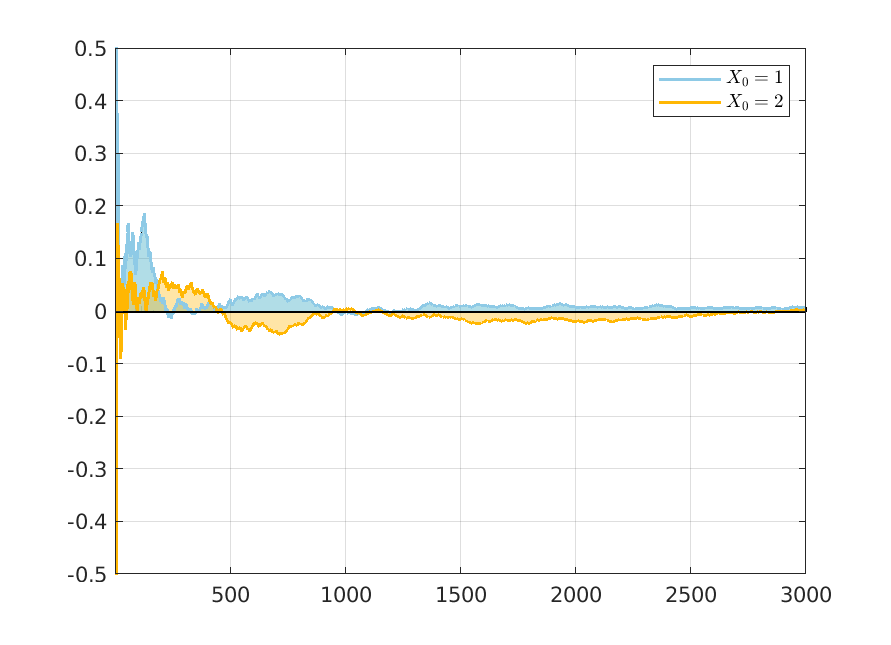
\includegraphics[width = 0.68\textwidth]{../figures/unemployment_dynamics.png}
    \caption{A Model of Unemployment Dynamics}
    \label{fig:unemployment}
\end{figure}
\end{frame}

\section{Functions}

\begin{frame}[fragile]
    \frametitle{User Defined Functions}
\begin{itemize}
    \item Commands are functions that take inputs and yield a result.
    \item In Matlab we can create our own functions just like in the mathematical sense.
    \item If $f(x) = 3x + 1$ then we can plug any $x$ and the result is $3x + 1$. This function in Matlab would be
\end{itemize}
\begin{lstlisting}
function [fx] = simple_function(x)
    fx = 3*x + 1;
end
\end{lstlisting}
\end{frame}

\begin{frame}[fragile]
    \frametitle{User Defined Functions}
\begin{itemize}
    \item The general structure of a function is
\begin{lstlisting}
function [out1,out2,...,outN] = name(in1,in2,...,inN)
    % Document the function. Author, inputs, outputs...
    Operations
    out1 = %operations to get out1;
    ...
    outN = %operations to get outN;
end
\end{lstlisting}
    \item Save the function as an \verb;.m; file in the working directory (or add to path).
    \item The name of the file \alert{\textbf{must be}} the name you assigned.
\end{itemize}
\end{frame}

\begin{frame}[fragile]
    \frametitle{User Defined Functions}
\begin{exercise}
Create a function called \verb;my_wave; that gives as output the plot of a sinusoidal wave. The function should take as arguments the parameters that will give the amplitude, the frequency, and the upper and lower bounds in which it will be plotted. By default, plot $1000$ points. Plot the sinusoidal wave with amplitude and frequency one for comparison. A sinusoidal wave $W$ with amplitude $A$ and frequency $f$ is computed as 
\[
W = A \sin(2\pi f x)
\]
\end{exercise}
\end{frame}

\begin{frame}[fragile]
    \frametitle{User Defined Functions}

A general function to compute a sine wave
\begin{lstlisting}
function [wave] = my_wave(A,freq,lb,ub)
    points = 1000;
    x = linspace(lb,ub,points);
    wave = A.*sin(2.*pi.*freq.*x);
    
    figure
    plot(x,wave,'--','LineWidth',1.3)
    hold on
    grid on
    plot(x,sin(x),'-','LineWidth',1.3)
    legend({'$A\sin(\omega x)$','$\sin(x)$'},'Interpreter','latex','Location','best')
    xlabel('$x$','Interpreter','latex')
    title(['Sinusoidal wave with amplitude ', num2str(A), ' and frequency ', num2str(freq)])
end
\end{lstlisting}
\end{frame}

\begin{frame}[fragile]
    \frametitle{Anonymous Functions}
    \begin{itemize}
      \item \href{https://www.mathworks.com/help/matlab/matlab_prog/anonymous-functions.html}{Anonymous functions} are functions \alert{\textit{not stored in an}\texttt{.m} \textit{file}}.
      \item These functions work within a script and they are stored in the workspace as \href{https://www.mathworks.com/help/matlab/ref/function_handle.html}{\texttt{function\_handle}} objects.
      \item To create an anonymous function that multiplies a number by two:
    \end{itemize}
  \begin{lstlisting}
  % Create the function
  bytwo = @(x) 2*x;
  % Call it
  a = bytwo(10);
  \end{lstlisting}
\end{frame}

\begin{frame}[fragile]
    \frametitle{Anonymous Functions}
    \begin{itemize}
        \item Note that these functions can contain only \alert{\textbf{one}} computable statement.
        \item Typically:
        \begin{itemize}
            \item Used for functions in the mathematical sense.
            \item Simple.
            \item Can take multiple inputs.
        \end{itemize}
    \end{itemize}
\end{frame}

\begin{frame}
    \frametitle{Anonymous Functions}
\begin{exercise}
Write the Rosenbrock function as an anonymous function and compute the value of $f(1,1), f(0,0), f(1,0)$, and $f(0,1)$. The Rosenbrock function is given by:
\[
f(x,y) = (1 - x)^2 + 100(y - x^2)^2    
\]
\end{exercise}
\end{frame}

\end{document}
